\chapter{Desarrollo de la secuencia didáctica 5E}\label{cap:desarrollo}

\textit{Este capítulo materializa el diseño del Capítulo 3: convierte cada fase en actividades concretas con su contenido, sus materiales y su evaluación, en torno a un mismo hilo conductor ---la determinación de la edad y el tamaño del universo---. Como soporte que da unidad al conjunto se \textbf{propone} una web interactiva, cuya finalidad, fundamento y articulación con las cinco fases se describen en §4.1; los detalles técnicos de la herramienta (arquitectura, programación y formatos de datos) no se recogen aquí, sino que quedan en los materiales de trabajo y se anexan a título de recurso. Los apartados que dependen de la implementación en el aula (curso 2026-2027) se señalan con la marca \textnormal{[por concretar]}.}

\section{Propuesta de una web interactiva como soporte de la secuencia}\label{sec:appweb}

\subsection{Finalidad y enfoque}

Como soporte que articula el desarrollo de la secuencia se \textbf{propone} una \textbf{web interactiva teórico-práctica} que reúne, en un único entorno, los recursos de las cinco fases 5E (Engage, Explore, Explain, Elaborate y Evaluate). El alumnado la utiliza a lo largo de toda la secuencia para acceder a la teoría adaptada a su nivel, realizar las actividades de forma interactiva ---medir, representar, ajustar y calcular---, obtener la constante de Hubble, la edad y el tamaño del universo. La web está disponible públicamente en \url{https://mrpiay.github.io/Cosmos5E/}, y su código fuente y materiales, en \url{https://github.com/mrpiay/Cosmos5E}.

El propósito pedagógico de la herramienta no es ofrecer resultados ya elaborados, sino \textbf{hacer tangible el proceso por el que la ciencia determina la edad y el tamaño del universo}: de la medida del corrimiento al rojo a la ley de Hubble, de ahí a $H_{0}$ y, finalmente, a la edad ($t \approx 1/H_{0}$) y al tamaño del universo observable. Frente a una calculadora convencional, que entrega un número sin mostrar su origen, la propuesta persigue \textbf{«abrir la caja negra»}: exhibir y explicar cada paso, cada término y cada unidad. De este modo la expansión del universo y la ley de Hubble-Lemaître se emplean como el \textbf{vehículo} que permite alcanzar el objetivo central ---edad y tamaño---, y la expansión acelerada, la energía y la materia oscura aparecen únicamente como \textbf{matiz} que refina y contextualiza la medida.

\begin{figure}[htbp]
\centering
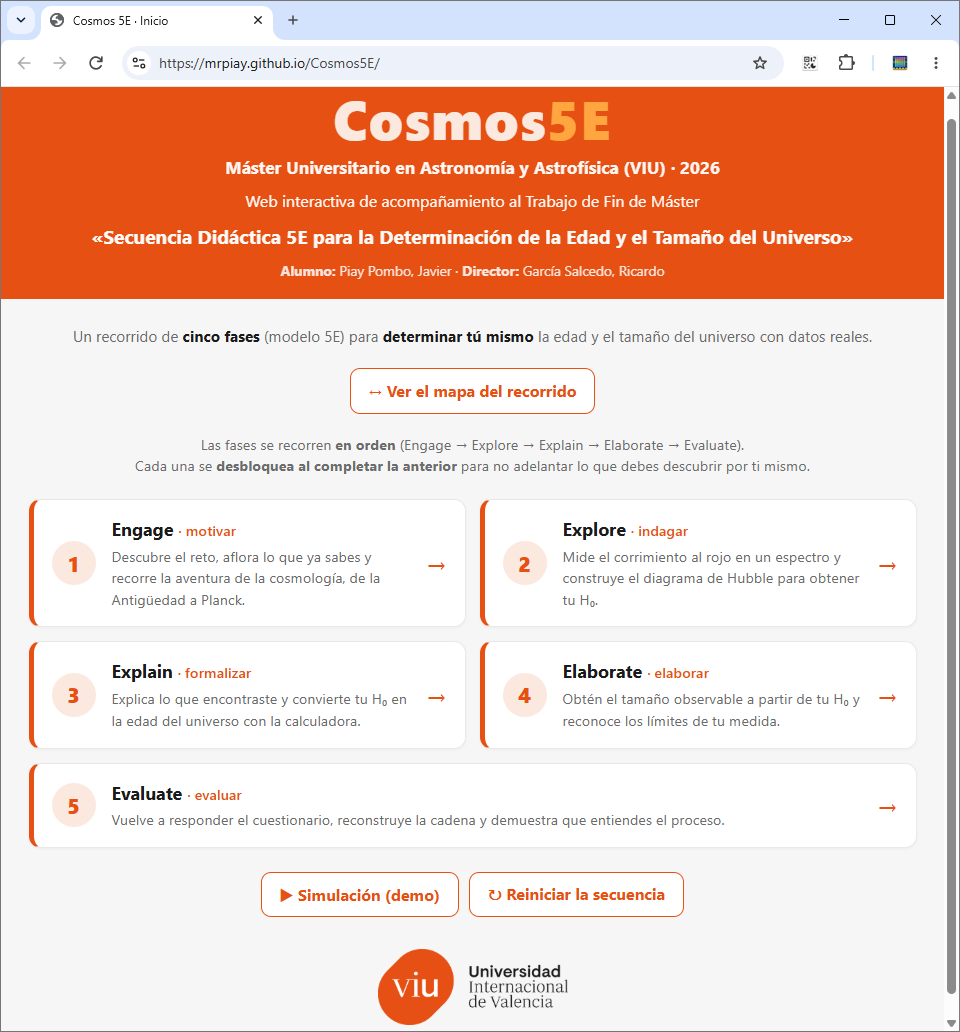
\includegraphics[width=0.85\textwidth]{./Images/web_v2_0_index.png}
\caption{Captura de la página de inicio de la web interactiva.}\label{fig:web-index}
\end{figure}

\subsection{Fundamento}

La web interactiva se fundamenta en la \textbf{revisión bibliográfica del Capítulo 2} ---de la que proceden los contenidos viables en el aula, las estrategias didácticas más eficaces y las ideas erróneas que conviene confrontar--- y emplea \textbf{datos y herramientas de acceso público}, citados a sus repositorios: las distancias del diagrama de Hubble proceden de la base de distancias independientes del corrimiento al rojo de NED \parencite{steer2017}, con el \textit{HST Key Project} \parencite{freedman2001} como contraste histórico; la calculadora se inspira en la de \textcite{wright2006}, reescrita en clave didáctica; y los valores cosmológicos actuales de referencia proceden de \textcite{planck2020}. Tanto la secuencia como la web interactiva se \textbf{inspiran} en los materiales y actividades docentes de la asignatura de Cosmología del Máster Universitario en Astronomía y Astrofísica de la VIU, \textbf{aprovechados y adaptados} al nivel de 2º de Bachillerato.

La transposición a este nivel implica sustituir lo inviable en el aula ---integrales de distancia cosmológica o software astronómico especializado no disponible en el aula--- por versiones interactivas, simplificadas y autónomas, centradas en el \textbf{régimen lineal} de la ley de Hubble ($v = H_{0}d$) y en la aproximación $t \approx 1/H_{0}$.

\subsection{Componentes}

La herramienta integra, para cada fase, cuatro tipos de componente:

\begin{itemize}
\item \textbf{Contenidos teóricos} breves y accesibles por concepto (escalas de espacio y tiempo, corrimiento al rojo, ley de Hubble-Lemaître, constante de Hubble, edad y tamaño del universo observable, ideas erróneas nucleares y naturaleza de la ciencia), acompañados de un \textbf{glosario} enlazado desde las actividades.
\item Una \textbf{calculadora didáctica} de $H_{0}$, la edad y el tamaño, concebida como una de las \textbf{herramientas clave} del conjunto: despliega la cadena de razonamiento paso a paso, explica cada término y \textbf{por qué interviene}, y hace visible la conversión de unidades que suele quedar oculta.
\item Un \textbf{diagrama de Hubble interactivo}, la otra herramienta clave: a partir de un conjunto de galaxias reales con su distancia y su velocidad de recesión, el alumnado ajusta una recta sobre los puntos representados y obtiene \textbf{su propio valor de $H_{0}$}. Las distancias proceden de métodos \textbf{independientes del corrimiento al rojo}, de modo que la ley de Hubble se «descubre» de forma genuina y no circular.
\item \textbf{La cadena de la medida}, una \textbf{secuencia de conceptos} visible en cada página de medida ---de Explore a Evaluate--- ($z \rightarrow v \rightarrow H_{0} \rightarrow$ edad $\rightarrow$ tamaño) que marca en qué punto del razonamiento se encuentra el alumnado y cómo cada concepto \textbf{conduce al siguiente} hasta comprender el valor final; no acumula números, sino que \textbf{encadena las ideas} del proceso.
\item Un \textbf{mapa del recorrido} accesible desde el inicio (Figura~\ref{fig:web-mapa}), que presenta el \textbf{propósito} y las \textbf{acciones} de cada fase y la pregunta que la enlaza con la siguiente ---una vista de conjunto para orientar al alumnado, sin adelantar las respuestas---.
\end{itemize}

\begin{figure}[htbp]
\centering
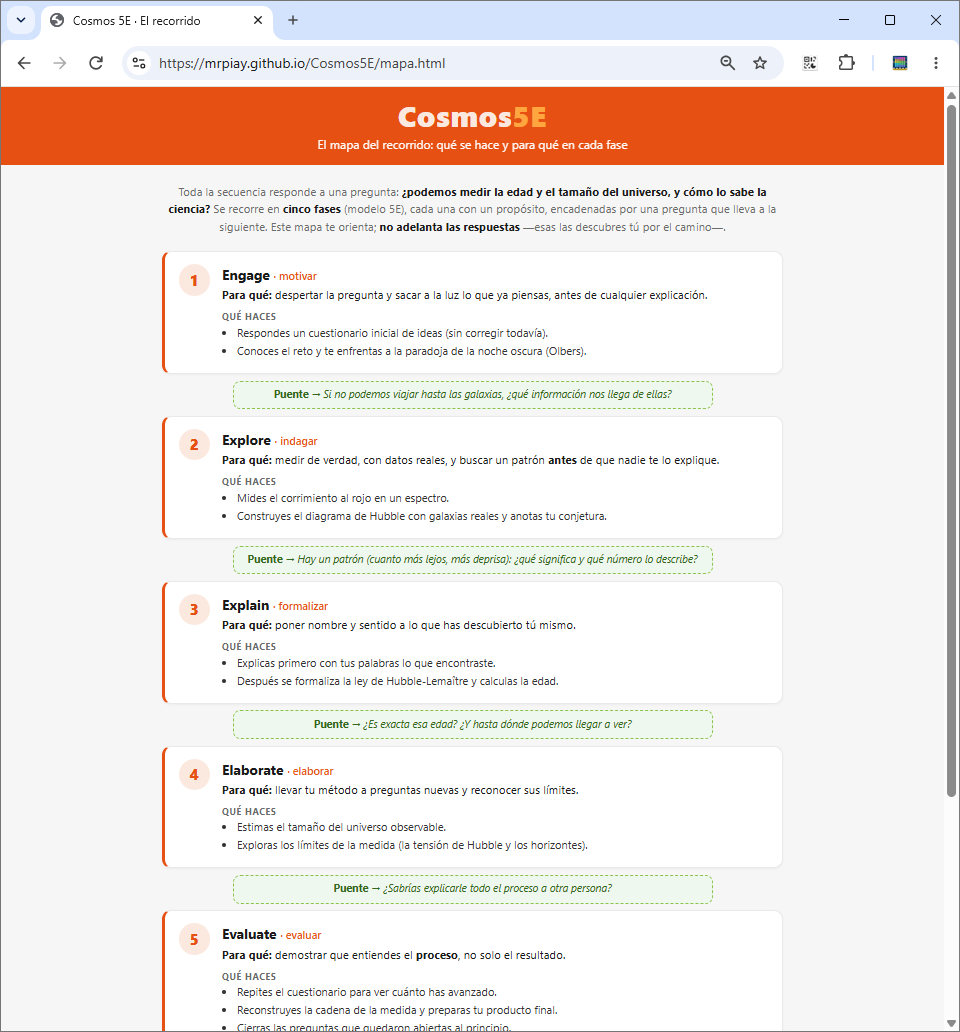
\includegraphics[width=0.85\textwidth]{./Images/web_v2_8_mapa.png}
\caption{Captura del \textbf{mapa del recorrido} de la secuencia 5E, accesible desde la página de inicio.}\label{fig:web-mapa}
\end{figure}

A ellos se suman los \textbf{instrumentos de evaluación} (cuestionario pre/post y rúbrica), descritos en §4.3.

\subsection{Principios de diseño}

La propuesta se rige por cuatro principios. \textbf{Autonomía y funcionamiento sin conexión}: construida con tecnologías web estándar, sin servidor ni dependencias externas, se abre en cualquier navegador sin instalación. \textbf{Adecuación al nivel}: vocabulario de 2º de Bachillerato y explicaciones antes que formalismo, con los valores actuales (Planck) como referencia pero dando prioridad al $H_{0}$ que \textbf{el propio alumnado mide}. \textbf{Equidad}: se mantiene una \textbf{alternativa no digital} (banda elástica y datos en papel) para quien no disponga de dispositivo. \textbf{Preguntar antes que explicar}: las cuestiones que Engage deja abiertas (los términos clave y la paradoja de Olbers) se mantienen vivas con \textbf{recordatorios} en cada fase ---«ya deberías poder responder\ldots»--- y se \textbf{cierran al final}, en Evaluate, cuando el alumnado ya tiene todas las piezas.

\subsection{Articulación con las cinco fases}

La herramienta se organiza como un recorrido por las cinco fases 5E; cada una integra su teoría, su actividad interactiva y su lugar en la cadena de la medida. La Tabla~\ref{tab:appfases} resume el encaje.

\begin{table}[ht]
\centering
\caption{Aportación de la herramienta en cada fase de la secuencia.}\label{tab:appfases}
\begin{tabularx}{\textwidth}{|>{\raggedright\arraybackslash}p{2.4cm}|>{\raggedright\arraybackslash}X|}
\hline
\rowcolor{naranja}
{\color{white}\textbf{Fase}} & {\color{white}\textbf{Aportación de la herramienta}} \\ \hline
Engage & Aflora las ideas previas con un \textbf{cuestionario conceptual} (sin adelantar respuestas); plantea el reto, define los términos clave, recorre la historia de la cosmología y provoca con la paradoja de Olbers. \\ \hline
Explore & En dos partes: medida del corrimiento al rojo en un espectro y \textbf{diagrama de Hubble interactivo} con galaxias reales, del que se obtiene el valor de $H_{0}$ (la pendiente). El alumnado \textbf{registra su conjetura} sobre lo observado, sin interpretarla todavía. \\ \hline
Explain & \textbf{Primero el alumnado explica} lo que encontró; después se formaliza la ley de Hubble-Lemaître y, con la \textbf{calculadora didáctica}, se obtiene la edad (cadena y conversión de unidades), con «rebobinar la expansión», el corrimiento cosmológico y el «calendario cósmico». \\ \hline
Elaborate & En dos partes: (1) el \textbf{tamaño} del universo observable ---radio de Hubble y por qué el observable real es mayor ($\sim$46\,000 millones de al)--- y una actividad de \textbf{transferencia} a otros valores de $H_{0}$; (2) los \textbf{límites} de la medida: tensión de Hubble, modelo $\Lambda$CDM y horizontes. \\ \hline
Evaluate & Cuestionario \textbf{post} (el mismo instrumento conceptual que el pre), repaso de la cadena ($z \rightarrow H_{0} \rightarrow$ edad $\rightarrow$ tamaño), \textbf{cierre de las preguntas abiertas del principio} (Olbers, edad, tamaño\ldots), lectura interactiva de las ecuaciones (clasificación por tipo) y guion del \textbf{producto final} con su rúbrica. \\ \hline
\end{tabularx}
\end{table}

\section{Desarrollo de las actividades por fase}\label{sec:desarrollo-detallado}

Esta sección desarrolla cada fase de la secuencia siguiendo la \textbf{plantilla común} definida en el Capítulo 3 (§3.7). El \textbf{diseño pedagógico} de cada fase ---el porqué de su función, la secuencia de actividades y las ecuaciones que introduce--- se ha detallado ya en el \textbf{recorrido por fases} de §\ref{sec:recorrido-fases}; para no duplicarlo, aquí cada ficha se centra en la \textbf{implementación en la web interactiva} y en los elementos operativos (contenido teórico al nivel del alumnado, interacción concreta, materiales, producto e indicadores de logro), remitiendo a aquel apartado para el desarrollo paso a paso. Todo ello se orienta a los objetivos de aprendizaje (OA1--OA7) y confronta las ideas erróneas de §3.5. Los materiales resultantes se recopilan en §4.6, y su versión completa constituye el guion de la web interactiva.

\subsection{Engage (motivar y aflorar ideas previas)}

\textbf{Pregunta que la abre:} ¿Tiene edad el universo? ¿Se puede determinar algo tan grande y lejano sin salir del aula?

\textbf{Objetivo(s) y OA:} despertar la pregunta motriz y aflorar las intuiciones sobre el espacio y el tiempo, diagnosticando concepciones \textit{(base para todos los OA; prepara OA1)}.

\textbf{Duración y agrupamiento:} 1 sesión (45 min); gran grupo con trabajo en pequeños grupos.

\subsubsection*{Qué sabemos e ideas previas}

Mediante un \textbf{cuestionario conceptual}, el alumnado responde, para cada concepto clave de la secuencia (año-luz, corrimiento al rojo, expansión, ley de Hubble, universo observable, etc.), una pregunta de opción múltiple ---con la opción \emph{«No lo sé / no lo tengo claro»} para quien no lo tenga claro, de modo que el pre-test queda completo---, \textbf{sin corrección a la vista} para no adelantar nada. Funciona a la vez como sondeo de \textbf{ideas previas} y como \textbf{pre-test conceptual}, el mismo instrumento que se repite en Evaluate.

\subsubsection*{Contenido teórico}

\textit{Nivel cualitativo, sin fórmulas.}
\begin{itemize}
\item \textbf{Qué significa determinar la edad y el tamaño:} la \textbf{edad} es el tiempo transcurrido desde el Big Bang ($\sim$13\,800 millones de años), no la de un astro concreto; el \textbf{tamaño} es el del universo \textbf{observable} ---la región cuya luz nos ha dado tiempo a alcanzar---, no el del universo total, que podría ser infinito.
\item \textbf{Medir sin viajar:} no vamos a las galaxias; leemos su \textbf{luz}, que transporta la información. Y como la luz tarda en llegar, \textbf{mirar lejos es mirar al pasado} (la luz como «máquina del tiempo»).
\item \textbf{La enormidad del tiempo cósmico, como pregunta abierta:} el universo es antiquísimo; ¿qué ha ocurrido en todo ese tiempo y cuándo? La pregunta se \textbf{planta aquí} y se responde en Explain (con el «calendario cósmico»).
\item \textbf{La cosmología como aventura (naturaleza de la ciencia):} nuestra visión del universo ha \textbf{cambiado} ---de la Tierra en el centro a la edad medida por el satélite Planck--- y cada salto llegó con una \textbf{tecnología} nueva para captar más luz.
\item \textbf{Paradoja de Olbers:} en un universo infinito, eterno y estático, \textbf{toda línea de visión} acabaría en la superficie de una estrella ---la debilidad de las lejanas se compensa con su mayor número--- y el cielo nocturno debería \textbf{brillar como el Sol}. Como no lo hace, alguna de esas premisas debe fallar: se plantea como \textbf{interrogante abierto} (¿cuál?), \textbf{sin resolver todavía} ---el alumnado lo retomará y cerrará al final---. La noche oscura es, así, un gancho hacia un universo \textbf{con historia}.
\end{itemize}

\subsubsection*{Desarrollo de la actividad}

El desarrollo paso a paso de esta fase ---reto y pregunta motriz, cuestionario conceptual (pre-test), definición de términos clave, aventura de la cosmología y paradoja de Olbers--- se detalla en el diseño de la secuencia (§\ref{sec:engage}). La paradoja de Olbers se plantea como provocación cualitativa \parencite{santos2014}, con apoyo opcional en la narrativa histórica \textit{Cosmic Times} \parencite{lochner2009,nunes2025}. Su implementación en la web se recoge a continuación.

\subsubsection*{Interacción en la web}

\begin{itemize}
\item \textbf{«El reto»:} una entrada que fija qué se va a determinar, por qué y para qué, con la pregunta motriz.
\item \textbf{Cuestionario conceptual:} por cada concepto, una \textbf{pregunta de opción múltiple} con distractores basados en ideas erróneas y una opción \emph{«No lo sé / no lo tengo claro»}; sin corrección, es el pre-test conceptual que se recupera y repite en Evaluate.
\item \textbf{Tarjetas de términos:} al pulsar cada término (edad, tamaño, universo observable, medir sin viajar) se revela «lo que suele creerse» frente a una \textbf{pista que despierta la curiosidad} ---una pregunta o una analogía que remite a fases posteriores---, no la definición completa.
\item \textbf{Línea de tiempo interactiva:} hitos de la historia de la cosmología (de la Antigüedad a Planck); al pulsar cada uno se revela qué cambió y la \textbf{tecnología} que lo permitió; los más recientes (expansión, fondo de microondas, edad) se plantean como \textbf{interrogantes} para no adelantar respuestas.
\item \textbf{Olbers interactivo:} un \textbf{control deslizante} que va llenando el cielo de estrellas (del mismo color) hasta \textbf{cubrirlo por completo}, mostrando que el fulgor surge de \textbf{tapar todos los huecos} y no de que cada estrella brille más; un \textbf{desplegable} aclara el porqué (el \textbf{brillo de superficie} no decae con la distancia). Se plantea como \textbf{interrogante} ---¿qué premisa falla?---, \textbf{sin resolverlo aquí}: la respuesta se construye a lo largo de la secuencia y se cierra en Evaluate.
\end{itemize}

\subsubsection*{Idea errónea que confronta}

Universo estático o eterno; Big Bang como «explosión»; dificultad para manejar las escalas espaciales y temporales.

\subsubsection*{Espacio--tiempo que se trabaja}

Primeras intuiciones; la enormidad del tiempo cósmico (planteada como pregunta abierta); la luz como puente entre distancia y tiempo ---mirar lejos es mirar al pasado---.

\subsubsection*{Materiales}

\begin{itemize}
\item \textbf{Hitos de la línea de tiempo} de la cosmología, con su tecnología asociada.
\item \textbf{Simulación interactiva de la paradoja de Olbers} (control local de «cobertura del cielo»).
\item \textbf{Cuestionario conceptual} de 15 ítems de opción múltiple (pre-test = post-test), con distractores basados en las ideas erróneas (§\ref{sec:instrumentos}).
\end{itemize}

\subsubsection*{Producto de la fase}

Primeras hipótesis sobre la edad y el tamaño del universo, y una idea clara de qué significan esos términos y de cómo la ciencia ha llegado a medirlos.

\subsubsection*{Indicadores de logro}

\begin{itemize}
\item Distingue qué significan la \textbf{edad} y el \textbf{tamaño} (observable) del universo, y reconoce que ese conocimiento ha \textbf{evolucionado} con la ciencia y la tecnología.
\item Expresa una hipótesis razonada sobre si el universo tiene edad y cómo podría determinarse.
\item Deja constancia de sus ideas previas (pre-test) para contrastarlas en Evaluate.
\end{itemize}

\subsubsection*{Puente a la siguiente fase}

Si no podemos ir hasta allí, ¿qué información nos llega de las galaxias? $\rightarrow$ \textbf{la luz}. Y queda rondando una \textbf{pregunta} ---¿qué ocurrió desde el Big Bang hasta hoy?--- que se responderá en Explain (con el «calendario cósmico»).

\begin{figure}[htbp]
\centering
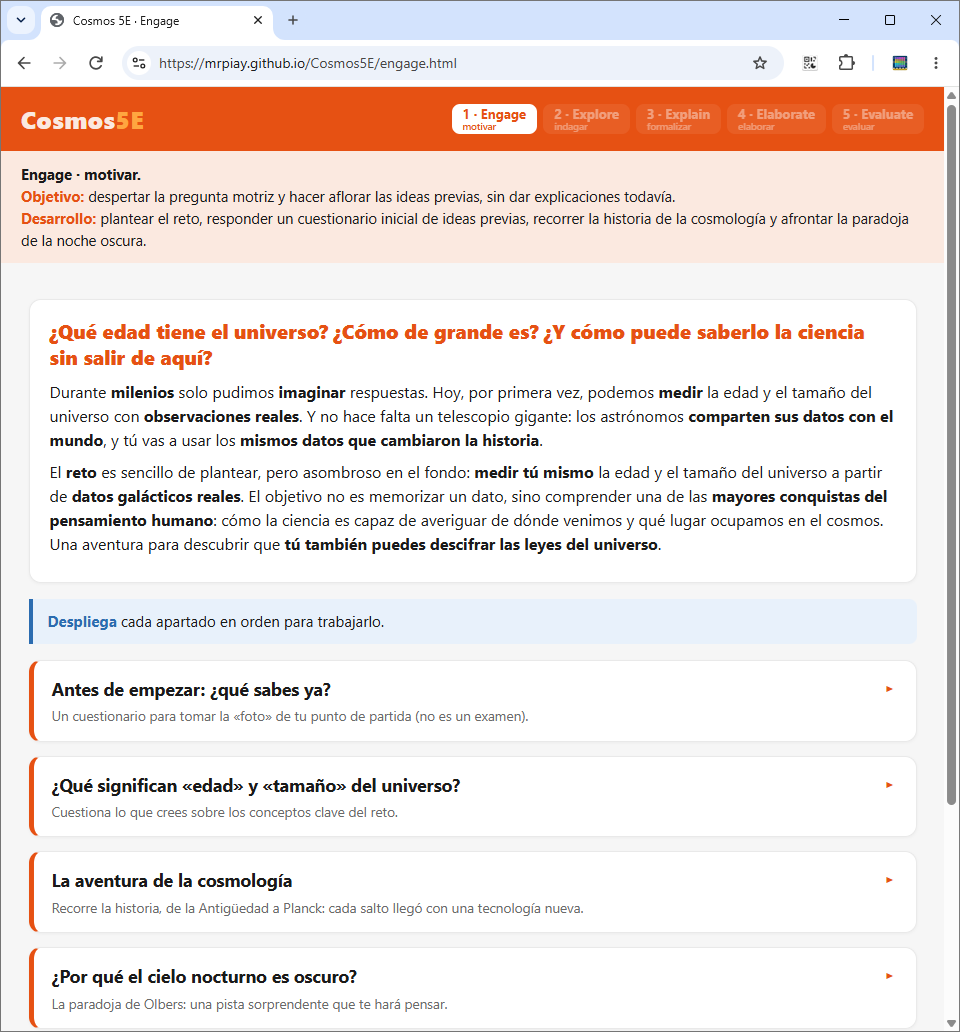
\includegraphics[width=0.82\textwidth]{./Images/web_v2_1_engage.png}
\caption{Captura de la sección \textbf{Engage} en la web interactiva.}\label{fig:web-engage}
\end{figure}

\subsection{Explore (indagación con datos)}

\textbf{Pregunta que la abre:} ¿Qué nos dice la luz de las galaxias? ¿Se mueven?

\textbf{Objetivo(s) y OA:} obtener $H_{0}$ a partir de la medida de la distancia y de la recesión \textit{(OA1, OA2, OA3)}.

\textbf{Duración y agrupamiento:} 2 sesiones (45 min); parejas o pequeños grupos.

\subsubsection*{Qué sabemos e ideas previas}

Concepto de \textbf{onda} y \textbf{efecto Doppler} (del sonido), qué es un \textbf{espectro}, la relación velocidad = distancia/tiempo y el \textbf{ajuste de una recta}.

\subsubsection*{Contenido teórico}

\begin{itemize}
\item \textbf{Cómo se miden las distancias} astronómicas (paralaje y candelas estándar), en breve, para que no sean «magia»; el \textbf{año-luz} como unidad del espacio.
\item \textbf{Corrimiento al rojo:} la luz de las galaxias llega «estirada» hacia el rojo; se mide con $z = \Delta\lambda/\lambda$ (desplazamiento relativo de una línea del espectro respecto a su longitud de onda en reposo).
\item \textbf{Velocidad de recesión:} para galaxias cercanas ($z$ pequeño), $v \approx c\,z$ \textit{(la web avisa de que esto solo vale a $z$ pequeño)}.
\item \textbf{El patrón velocidad--distancia:} al representar $v$ frente a $d$, los puntos se alinean formando una recta cuya \textbf{pendiente} es la medida que se busca (se la llamará $H_{0}$). En Explore \textbf{no se nombra aún la ley ni se interpreta el patrón} ---qué significa o por qué la recta pasa por el origen---: eso se reserva para Explain.
\end{itemize}

\subsubsection*{Desarrollo de la actividad}

El desarrollo paso a paso de las dos actividades de esta fase ---medir el corrimiento al rojo ($z = \Delta\lambda/\lambda$, $v = c\,z$) y descubrir la relación distancia--velocidad construyendo el diagrama de Hubble y registrando la conjetura--- se detalla en el diseño de la secuencia (§\ref{sec:explore}). En el aula puede apoyarse con banda elástica y \textit{Tracker} \parencite{suarez2025} o con datos reales en hoja de cálculo \parencite{cardona2016,hyde2021}. Su implementación en la web se recoge a continuación.

\subsubsection*{Interacción en la web}

\begin{itemize}
\item \textbf{Explorar el corrimiento al rojo:} sobre una \textbf{galaxia hipotética}, el alumnado \textbf{arrastra} la línea de emisión (H$\alpha$) y ve \textbf{en vivo} cómo su desplazamiento se traduce en $z = \Delta\lambda/\lambda$ y $v = c\,z$; se plantea como \textbf{pregunta abierta} si de verdad es un efecto Doppler ---se resolverá en Explain---.
\item \textbf{Diagrama de Hubble interactivo (la actividad central):} el alumnado ajusta la recta sobre los puntos ya representados (arrastrando su pendiente o con «ajuste automático»); la web muestra su valor ---la pendiente--- y las barras de error de los puntos dejan ver la incertidumbre de los datos. Ese es el valor que llevará a Explain, \textbf{todavía sin interpretar} qué significa.
\item \textbf{Registro de la conjetura:} al terminar, un formulario recoge qué patrón ve el alumnado, qué cree que significa la pendiente, por qué algunas galaxias se salen y qué ocurriría al «rebobinar» el tiempo; hay que completarlo para poder continuar, y se recupera en Explain.
\item \textbf{Datos de partida:} 15 galaxias reales de 15 a 153 Mpc con distancia independiente del corrimiento al rojo y velocidad $v = c\,z$; el ajuste con las de flujo limpio ($v > 3000$ km/s) da $H_{0} \approx 70$ y, por tanto, $1/H_{0} \approx 14$ Gyr. Se incluyen a propósito galaxias cercanas dispersas (NGC 4536, NGC 4639\ldots) para discutir las velocidades peculiares. Fuente: NED-D \parencite{steer2017}, con el \textit{HST Key Project} \parencite{freedman2001} como contraste.
\item \textbf{Alternativa no digital} (§4.4): la misma actividad con banda elástica y datos en papel.
\end{itemize}

\subsubsection*{Idea errónea que confronta}

«Todo corrimiento al rojo es efecto Doppler ordinario»; «la expansión es el movimiento propio de las galaxias por el espacio».

\subsubsection*{Espacio--tiempo que se trabaja}

La medida del \textbf{espacio}: distancias astronómicas y el año-luz.

\subsubsection*{Materiales}

\begin{itemize}
\item \textbf{Espectro(s)} de trabajo: espectro de una galaxia (real o representativa) con una línea identificable ---p.\,ej. H$\alpha$--- para medir su corrimiento al rojo $z$.
\item \textbf{Dataset del diagrama de Hubble:} 15 galaxias (NED-D) con distancia, velocidad $v = c\,z$ e incertidumbre.
\item Herramienta de \textbf{ajuste de recta} (web) y su alternativa con \textbf{banda elástica} (no digital).
\end{itemize}

\subsubsection*{Producto de la fase}

El diagrama de Hubble del alumnado y su valor de $H_{0}$ (con incertidumbre).

\subsubsection*{Indicadores de logro}

\begin{itemize}
\item Mide $z$ correctamente a partir de un espectro y obtiene $v = c\,z$.
\item Construye el diagrama de Hubble y obtiene un $H_{0}$ razonable, con noción de incertidumbre.
\item Distingue la recesión por expansión del espacio del movimiento propio de la galaxia.
\end{itemize}

\subsubsection*{Puente a la siguiente fase}

Hay un patrón ($v$ crece con $d$): ¿qué significa y qué número lo describe? $\rightarrow$ la constante de Hubble y qué podemos calcular con ella.

\begin{figure}[htbp]
\centering
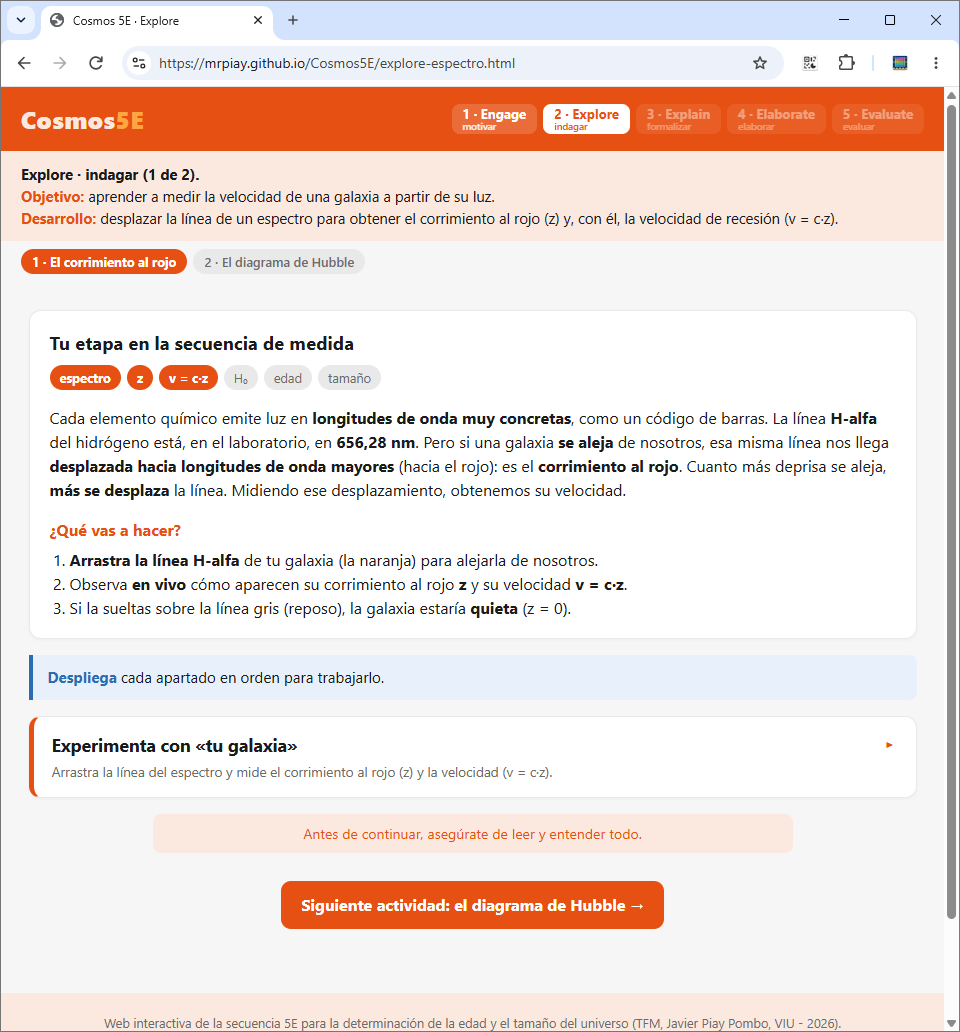
\includegraphics[width=0.48\textwidth]{./Images/web_v2_2_espectro.png}\hfill
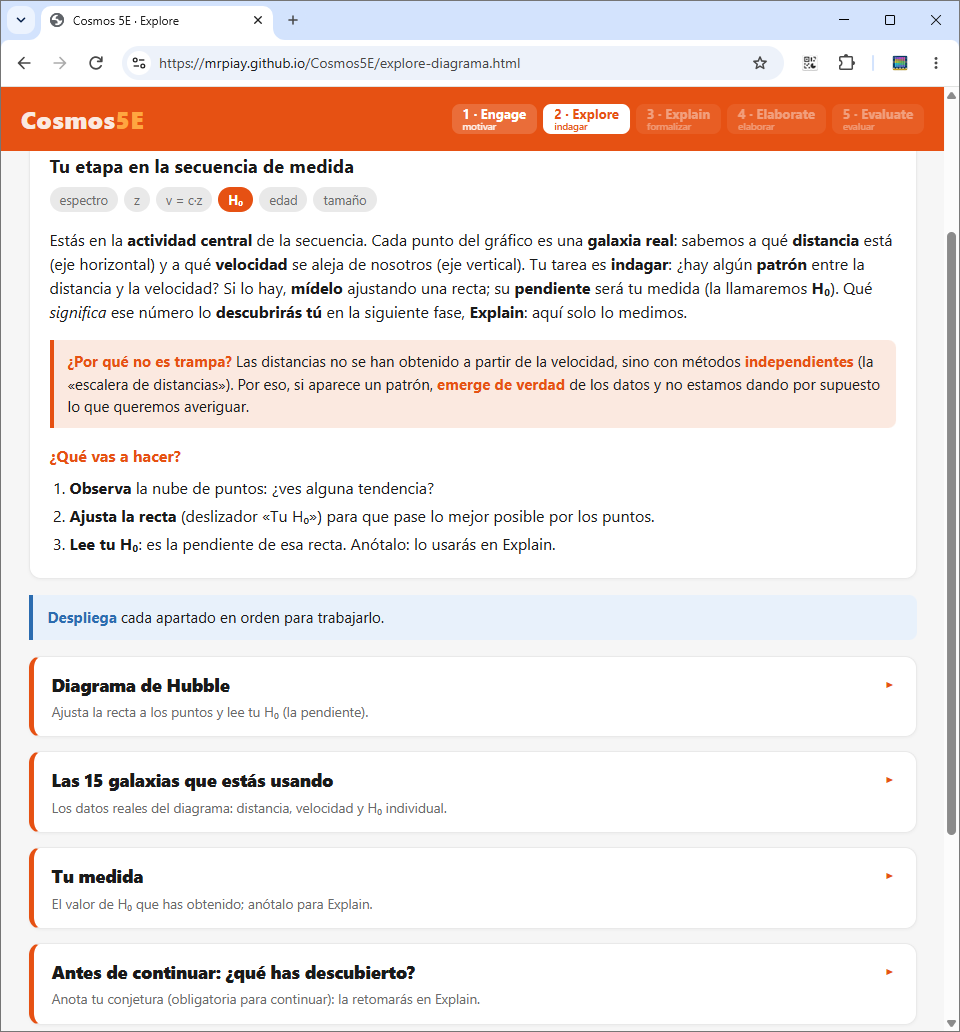
\includegraphics[width=0.48\textwidth]{./Images/web_v2_3_diagrama.png}
\caption{Capturas de la sección \textbf{Explore} en la web interactiva: espectro (izquierda) y diagrama de Hubble (derecha).}\label{fig:web-explore}
\end{figure}

\subsection{Explain (formalizar el concepto)}

\textbf{Pregunta que la abre:} ¿Qué significa que la velocidad aumente con la distancia? ¿Qué es $H_{0}$ y qué podemos calcular con él?

\textbf{Objetivo(s) y OA:} conectar $H_{0}$ con la edad del universo, situarla en perspectiva y formalizar el corrimiento al rojo \textit{(OA2, OA3, OA4)}.

\textbf{Duración y agrupamiento:} 1 sesión (45 min); gran grupo con resolución individual.

\subsubsection*{Qué sabemos e ideas previas}

El \textbf{valor} (la pendiente) y la \textbf{recta $v$--$d$} que el propio alumnado obtuvo en Explore, y la \textbf{conjetura} que anotó allí.

\subsubsection*{Contenido teórico}

\begin{itemize}
\item \textbf{Qué es $H_{0}$ de verdad:} el \textbf{ritmo de expansión} del universo (cuánta velocidad de recesión por cada unidad de distancia); unidades km/s/Mpc.
\item \textbf{De $H_{0}$ a la edad:} por \textbf{extrapolación lineal} de la tasa de expansión actual, el tiempo transcurrido desde el Big Bang sería $t \approx 1/H_{0}$ (\textbf{tiempo de Hubble}), un valor del \textbf{orden} de la edad.
\item \textbf{Conversión de unidades} (explícita y central): con $1\ \text{Mpc} = 3{,}086\cdot10^{19}$ km, $1/H_{0} \approx 4{,}4\cdot10^{17}$ s $\approx 14\,000$ millones de años (la web lo muestra paso a paso).
\item \textbf{Por qué $1/H_{0}$ es la edad del universo:} al \textbf{rebobinar} la expansión, las \textbf{distancias entre todas las galaxias se reducen a la vez} ---las lejanas van proporcionalmente más rápido---, hace $\sim 1/H_{0}$, hasta un estado inicial muy denso y caliente (el Big Bang), \textbf{sin un punto ni un centro privilegiado}. Es una \textbf{distancia $\div$ velocidad de recesión} ($d/v$) ---la edad del \textbf{universo entero}---, y no el tiempo que tardó en llegarnos la luz de una galaxia ($d/c$, mucho menor).
\item \textbf{El corrimiento al rojo de la luz es siempre cosmológico:} la luz llega estirada porque \textbf{el espacio se estira} mientras viaja, no porque la galaxia «vuele» a través de él. En galaxias cercanas ($z$ pequeño), la \textbf{fórmula del Doppler} $v = c\,z$ da el número correcto y se usa como \textbf{atajo}, pero \textbf{cualitativamente es incorrecta}; solo el pequeño movimiento propio (velocidades peculiares) es un Doppler real \parencite{xu2018,possel2020,marshall2022}.
\item \textbf{La edad, en perspectiva (calendario cósmico):} esos $\sim$14\,000 millones de años son inabarcables; comprimir toda la historia del universo en un año hace tangible la escala ---la humanidad ocupa los últimos segundos--- y responde a la \textbf{gran pregunta} planteada en Engage \parencite{colantonio2019}.
\end{itemize}

\subsubsection*{Desarrollo de la actividad}

El desarrollo paso a paso de esta fase ---recuperar y poner en común la explicación del alumnado; formalizar $v = H_{0}d$ e identificar la pendiente como $H_{0}$; deducir y calcular $t \approx 1/H_{0}$ con la conversión de unidades; recorrer la historia de la expansión (hacia adelante y atrás); distinguir el corrimiento al rojo cosmológico del Doppler; y poner la edad en perspectiva con el calendario cósmico--- se detalla en el diseño de la secuencia (§\ref{sec:explain}). Su implementación en la web se recoge a continuación.

\subsubsection*{Interacción en la web}

\begin{itemize}
\item \textbf{«Tu explicación» (antes de nada):} la web recupera la conjetura de Explore y pide al alumnado que explique con sus palabras lo que encontró; \textbf{hay que guardarla para poder revelar la explicación científica}, de modo que se razona primero y la formalización llega después.
\item \textbf{Calculadora didáctica (la herramienta central de esta fase):} el alumnado introduce su $H_{0}$ (el de Explore) y ve salir la edad, con la cadena y la conversión de unidades a la vista, término a término.
\item \textbf{«La historia del universo» (interactivo):} un deslizador recorre la historia ---hacia adelante y hacia atrás--- sobre un \textbf{trozo de espacio} representado como una textura que cambia de escala: al rebobinar, el espacio se \textbf{comprime por igual en todas partes} (sin un centro) hasta un estado \textbf{denso y caliente} anterior a las galaxias; al avanzar, se forman las galaxias y, más tarde, aparecemos \textbf{nosotros} (la Tierra, un «punto azul pálido»), que las vemos ya muy lejos. Hace tangible que $1/H_{0}$ marca el \textbf{orden} de la edad y que las estructuras ---y nosotros--- se formaron mucho después del inicio.
\item \textbf{«El corrimiento al rojo de la luz»:} explica que el estiramiento es \textbf{siempre cosmológico} y que $v = c\,z$ es solo un \textbf{atajo} numérico válido en galaxias cercanas ($z$ pequeño), cualitativamente incorrecto; lo distingue de las velocidades peculiares (Doppler real) y recuerda que los \textbf{sistemas ligados} (galaxias, Sistema Solar, personas) no se expanden.
\item \textbf{«Calendario cósmico» (cierre):} tras estimar la edad, un deslizador comprime toda la historia del universo en un año y muestra cuándo ocurre cada suceso ---la humanidad, en los últimos segundos---; \textbf{responde la gran pregunta} planteada en Engage.
\end{itemize}

\subsubsection*{Idea errónea que confronta}

Corrimiento al rojo = Doppler; los sistemas ligados (galaxias, Sistema Solar, personas) se expanden.

\subsubsection*{Espacio--tiempo que se trabaja}

La \textbf{unión de ambos}: de una velocidad y una distancia se obtiene un tiempo (la edad); mirar lejos es mirar al pasado. La escala de esa edad se hace tangible con el \textbf{calendario cósmico}.

\subsubsection*{Materiales}

\begin{itemize}
\item \textbf{Calculadora didáctica} (web).
\item Gráfico interactivo \textbf{«rebobinar la expansión»} (web).
\item Recurso \textbf{«el corrimiento al rojo de la luz»} (web): $v = c\,z$ como atajo frente al estiramiento cosmológico.
\item \textbf{Datos del calendario cósmico} (sucesos y su fecha en el «año» del universo).
\end{itemize}

\subsubsection*{Producto de la fase}

Estimación razonada de la edad del universo (a partir de su $H_{0}$), con la conversión de unidades hecha.

\subsubsection*{Indicadores de logro}

\begin{itemize}
\item Interpreta $H_{0}$ como ritmo de expansión (no como una velocidad sin más).
\item Deduce y calcula $t \approx 1/H_{0}$ con la conversión de unidades correcta.
\item Explica que el corrimiento al rojo cosmológico es estiramiento del espacio y que los sistemas ligados no se expanden.
\item Explica por qué $1/H_{0}$ es la edad del universo ($d/v$) y no el tiempo de viaje de la luz de un objeto ($d/c$).
\item Sitúa la edad estimada en perspectiva con el calendario cósmico.
\end{itemize}

\subsubsection*{Puente a la siguiente fase}

¿Es exacta esa edad? ¿Y hasta dónde podemos ver? $\rightarrow$ los límites de la estimación y el tamaño del universo observable.

\begin{figure}[htbp]
\centering
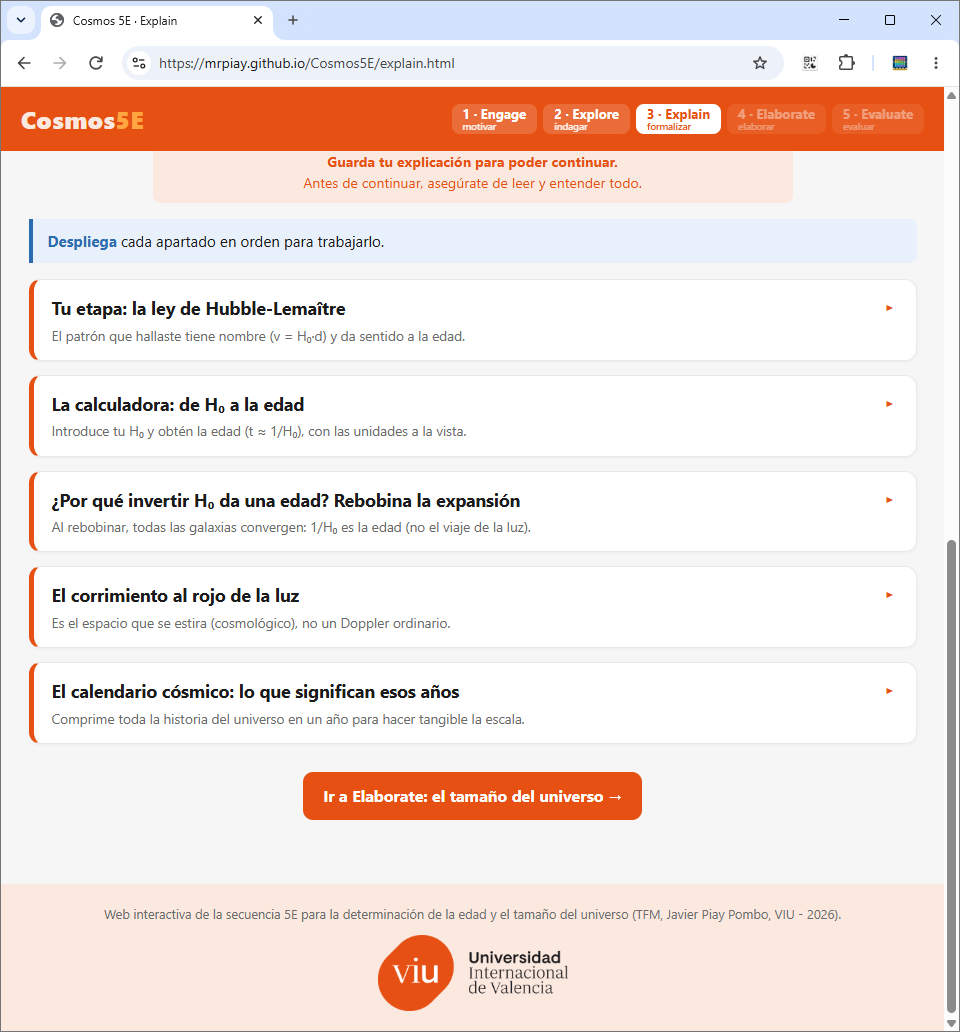
\includegraphics[width=0.82\textwidth]{./Images/web_v2_4_explain.png}
\caption{Captura de la sección \textbf{Explain} en la web interactiva.}\label{fig:web-explain}
\end{figure}

\subsection{Elaborate (refinar y contextualizar la medida)}

\textbf{Pregunta que la abre:} ¿Qué tamaño tiene lo observable y qué límites tiene nuestra estimación?

\textbf{Objetivo(s) y OA:} refinar la medida y reconocer sus límites (calcular el \textbf{tamaño} del universo observable y entender por qué $t \approx 1/H_{0}$ es solo una primera aproximación) y valorar que la ciencia avanza discutiendo modelos y teorías \textit{(OA4, OA5, OA6, OA7)}.

\textbf{Duración y agrupamiento:} 2 sesiones (45 min c/u); pequeños grupos con debate en gran grupo. La \textbf{primera} se centra en el \textbf{tamaño observable} (radio de Hubble, su relación con el radio observable y la CMB); la \textbf{segunda}, en los \textbf{límites y matices} (alcance de $1/H_{0}$, horizonte de sucesos ---un paso más allá---, $\Lambda$CDM y tensión de Hubble).

\subsubsection*{Qué sabemos e ideas previas}

La \textbf{edad estimada} ($t \approx 1/H_{0}$) y el \textbf{valor de $H_{0}$} obtenidos en las fases anteriores.

\subsubsection*{Contenido teórico}

\begin{itemize}
\item \textbf{El radio de Hubble (escala característica de distancia):} $R \approx c\,(1/H_{0}) = c/H_{0}$ ($\approx 14\,000$ millones de años-luz con $H_{0} \approx 70$); \emph{no} es el tamaño del universo observable.
\item \textbf{Matiz (para no enseñar un error):} el radio observable real es mayor ($\sim$46\,000 millones de años-luz; el diámetro, $\sim$92\,000) porque el espacio se estiró mientras la luz viajaba; en bachillerato se estima solo el orden de magnitud, pues el cálculo exacto exige integrar la expansión (fuera del alcance) \parencite{linton2012}.
\item \textbf{El alcance de $t \approx 1/H_{0}$:} da una escala del \textbf{orden de la edad}; el valor \textbf{preciso} depende tanto del \textbf{valor de $H_{0}$} como de la \textbf{historia de la expansión} $H(t)$. Una fuente de incertidumbre muy debatida es el propio $H_{0}$ ---de ahí la tensión de Hubble---.
\item \textbf{El modelo estándar y la naturaleza de la ciencia:} el consenso actual, $\Lambda$CDM, describe un universo \textbf{plano} y de \textbf{unos 13\,800 millones de años}, dominado por la \textbf{energía oscura} ($\Lambda$, $\sim$68\,\%, que acelera la expansión) y la \textbf{materia oscura} (CDM, $\sim$27\,\%, que gravita), con solo un $\sim$5\,\% de materia ordinaria; encaja con observaciones independientes (fondo cósmico de microondas, supernovas y distribución de galaxias). No es un dogma: persiste la \textbf{tensión de Hubble} ---distintos métodos dan valores de $H_{0}$ algo distintos y, por tanto, edades algo distintas--- y hay teorías alternativas en la frontera (p.\,ej. MOND o la gravedad conforme) \parencite{planck2020}.
\item \textbf{Materia oscura $\neq$ energía oscura} (conceptos distintos: una «pesa», la otra «acelera»).
\item \textbf{El último horizonte (los límites de lo observable) ---un paso más allá---:} el universo observable \textbf{no crece sin límite} ---su radio tiende a un valor máximo---; más allá del \textbf{horizonte de sucesos cosmológico} ($\sim$16\,000 millones de años-luz) la expansión acelerada impide que la luz que las galaxias emiten \textbf{hoy} llegue jamás. Es un horizonte \textbf{distinto} de la esfera de Hubble ($\sim$14) y del universo observable ($\sim$46), y enlaza con la paradoja de Olbers de Engage.
\end{itemize}

\subsubsection*{Desarrollo de la actividad}

El desarrollo paso a paso de las dos partes de esta fase ---\textbf{el tamaño observable} (radio de Hubble $c/H_{0}$ y por qué el observable real es mayor) y \textbf{los límites de la medida} (transferencia a otros valores de $H_{0}$, tensión de Hubble y modelo estándar $\Lambda$CDM)--- se detalla en el diseño de la secuencia (§\ref{sec:elaborate}). La energía oscura aparece solo como \textbf{matiz} de la medida \parencite{hyde2021,pereira2019,raymundo2022}. Su implementación en la web se recoge a continuación.

\subsubsection*{Interacción en la web}

\begin{itemize}
\item \textbf{El tamaño observable, en dos pasos:} primero el \textbf{radio de Hubble} $R \approx c/H_{0}$ como \textbf{escala característica}; después, un \textbf{esquema interactivo} en el que se elige la \textbf{distancia de la fuente} (de una galaxia cercana al fondo de microondas) y, al avanzar el tiempo, el espacio se estira \textbf{en todas partes} (una rejilla) y la galaxia se aleja, con \textbf{cifras que se actualizan} ---camino recorrido, expansión, distancias y la \textbf{razón distancia hoy $\div$ camino}--- que hacen ver que la luz de las fuentes lejanas \textbf{al principio pierde terreno} y que esa razón \textbf{crece con la distancia} (de $\sim$1{,}2 en las cercanas a $\sim$3{,}3 en el borde): \textbf{no es una regla fija}, sino que proviene de la historia de la expansión. Así el \textbf{radio observable} ($\sim$46\,000 millones de años-luz; el diámetro, $\sim$92\,000) resulta \textbf{bastante mayor} que el radio de Hubble, aunque son \textbf{magnitudes distintas}. Se acompaña de una \textbf{derivación cualitativa con el fondo cósmico de microondas} (su $z \approx 1100$) que explica por qué el radio observable supera a $c \times$ edad.
\item \textbf{El modelo estándar $\Lambda$CDM en breve:} una ficha que resume qué contiene el universo ---con la distinción entre \textbf{materia oscura} («pesa», gravita) y \textbf{energía oscura} («acelera» la expansión)--- y que su expansión se \textbf{acelera}, como contexto de la medida.
\item \textbf{La tensión de Hubble:} se contrastan dos valores típicos ($\sim$67 de Planck y $\sim$73 de supernovas) y sus edades algo distintas, como ejemplo de incertidumbre y debate abierto (el efecto numérico de cambiar $H_{0}$ ya se explora en «Transferencia»).
\item \textbf{Sección de cierre «Un último horizonte» (un paso más allá):} distingue los \textbf{tres radios} ---esfera de Hubble ($\sim$14), horizonte de sucesos ($\sim$16) y universo observable ($\sim$46)--- y, con un \textbf{diagrama} y un \textbf{ejemplo numérico paso a paso} (un \textbf{modelo didáctico simplificado}, no una descripción exacta: el fotón avanza a $c$ y el espacio se expande un porcentaje fijo por paso), muestra por qué la luz que las galaxias más lejanas emiten \textbf{hoy} \textbf{nunca} nos alcanzará ---sin recurrir a velocidades superlumínicas--- y por qué el tamaño observable tiende a un techo; cierra retomando el «tercer factor» de la paradoja de Olbers.
\item \textbf{Transferencia:} el alumnado introduce otros valores de $H_{0}$ (Planck, supernovas, otro grupo) y compara al instante las edades y tamaños resultantes.
\end{itemize}

\subsubsection*{Idea errónea que confronta}

$t = 1/H_{0}$ como valor exacto; el radio observable como $c \times$ edad; energía oscura como sustancia o fuerza; confusión materia/energía oscura; la recesión superlumínica (creer que las galaxias «se alejan más rápido que la luz»); la ciencia como conjunto de hechos cerrados.

\subsubsection*{Espacio--tiempo que se trabaja}

El \textbf{tamaño} (espacio) del universo observable y los límites de la medida.

\subsubsection*{Materiales}

\begin{itemize}
\item \textbf{Calculadora didáctica} (paso «tamaño»), \textbf{deslizador} de la tensión de Hubble y \textbf{ficha del modelo $\Lambda$CDM}.
\item \textit{(Opcional)} datos de supernovas o simulador de energía oscura.
\end{itemize}

\subsubsection*{Producto de la fase}

Estimación refinada del tamaño observable y una explicación de los límites de la estimación.

\subsubsection*{Indicadores de logro}

\begin{itemize}
\item Calcula el tamaño observable (orden de magnitud) a partir de su $H_{0}$.
\item Reconoce que $1/H_{0}$ es una \textbf{estimación muy buena} de la edad (y que su valor depende del $H_{0}$ adoptado) y explica por qué el tamaño observable real es mayor que $c \times$ edad.
\item Distingue la materia oscura de la energía oscura.
\item Argumenta que la ciencia progresa debatiendo entre modelos (tensión de Hubble, alternativas, consenso $\Lambda$CDM).
\end{itemize}

\subsubsection*{Puente a la siguiente fase}

¿Sabríamos explicar todo el proceso a otra persona? $\rightarrow$ demostrar que entendemos el proceso, no solo el resultado.

\begin{figure}[htbp]
\centering
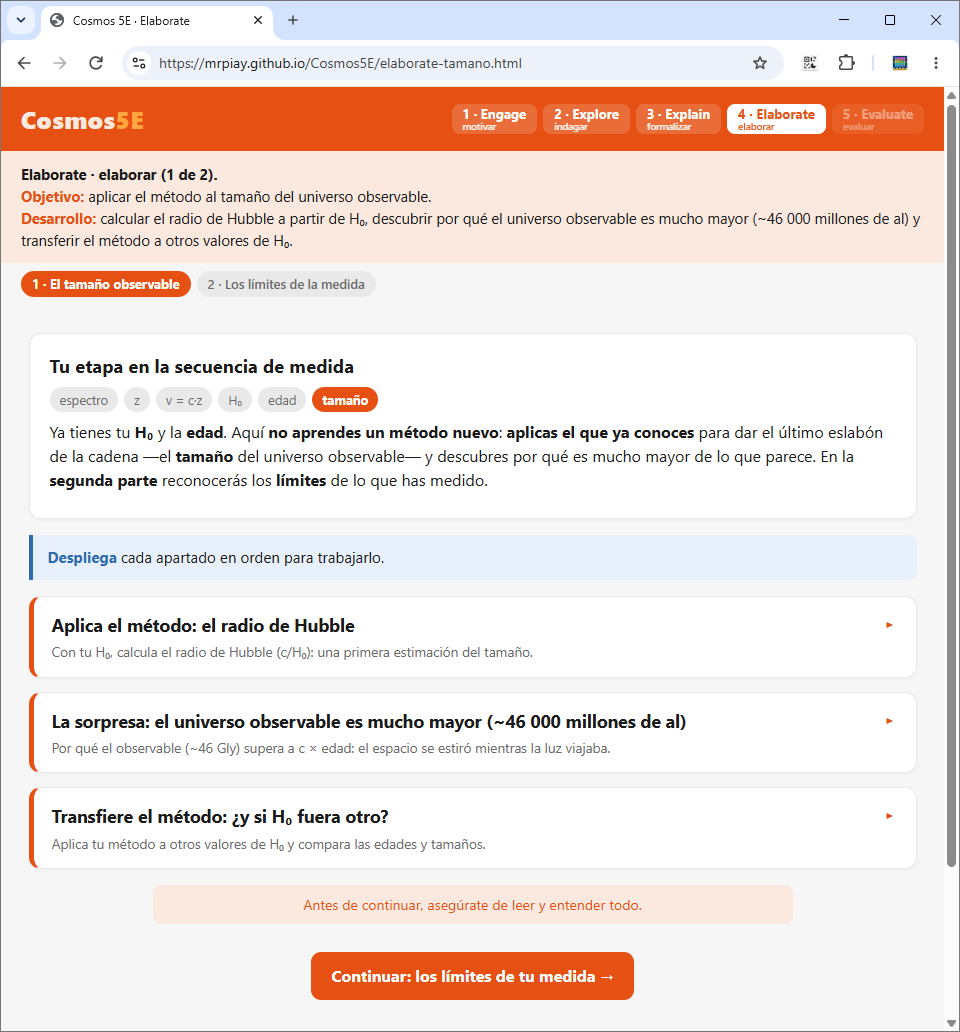
\includegraphics[width=0.82\textwidth]{./Images/web_v2_5_elaborate_tamano.png}
\caption{Captura de la sección \textbf{Elaborate}, parte 1: el tamaño del universo observable.}\label{fig:web-elaborate-tamano}
\end{figure}

\begin{figure}[htbp]
\centering
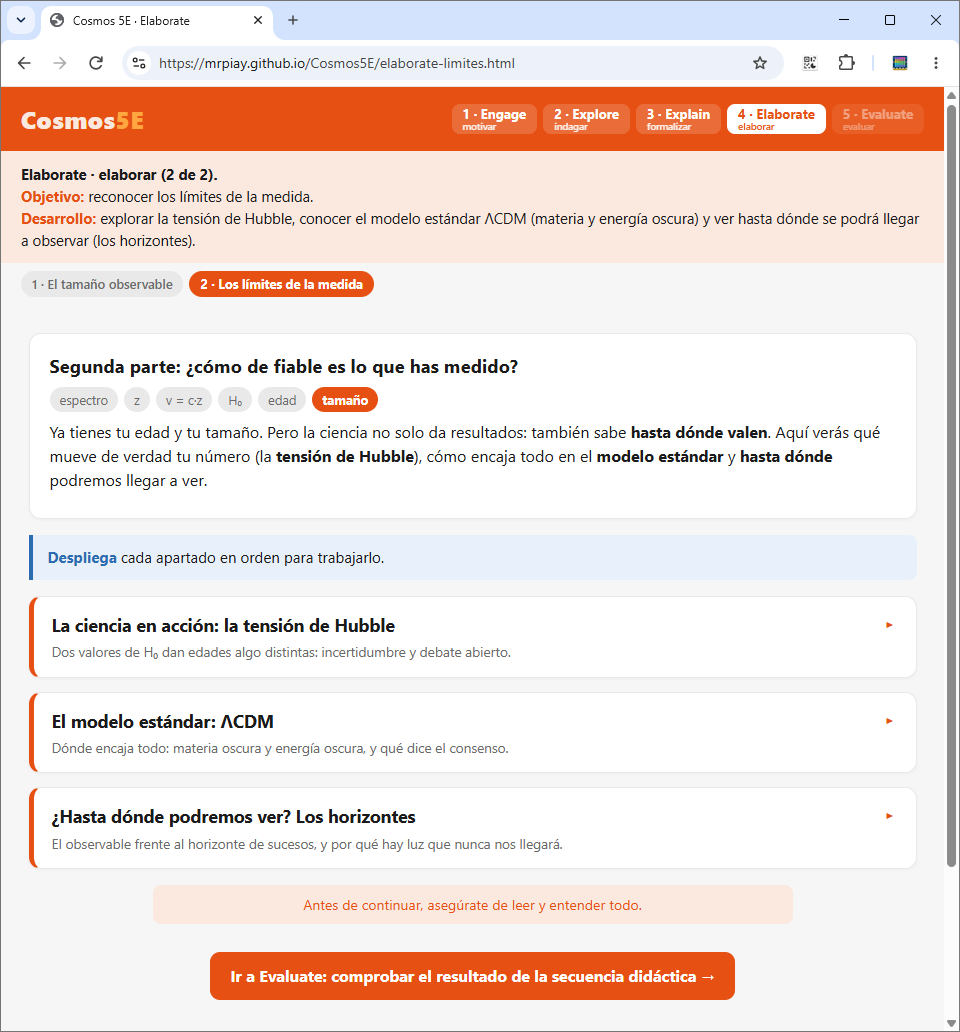
\includegraphics[width=0.82\textwidth]{./Images/web_v2_6_elaborate_limites.png}
\caption{Captura de la sección \textbf{Elaborate}, parte 2: los límites de la medida (tensión de Hubble, $\Lambda$CDM y horizontes).}\label{fig:web-elaborate-limites}
\end{figure}

\subsection{Evaluate (evaluar la comprensión)}

\textbf{Pregunta que la abre:} ¿Cómo hemos medido la edad y el tamaño del universo?

\textbf{Objetivo(s) y OA:} medir el aprendizaje y el \textbf{cambio conceptual} \textit{(OA1--OA7)}.

\textbf{Duración y agrupamiento:} 1 sesión (45 min); individual (cuestionario) y gran grupo (puesta en común).

\subsubsection*{Qué sabemos e ideas previas}

Todo el recorrido conceptual de la secuencia ($z \rightarrow H_{0} \rightarrow$ edad $\rightarrow$ tamaño).

\subsubsection*{Contenido teórico}

No se introduce teoría nueva: se \textbf{sintetiza e integra} el recorrido ---espacio (tamaño) y tiempo (edad) como magnitudes \textbf{inferidas y aproximadas}, no como datos absolutos---, reforzando la naturaleza de la ciencia (medir es inferir con modelos y aproximaciones, y revisar).

\subsubsection*{Desarrollo de la actividad}

El desarrollo paso a paso de esta fase ---cuestionario post y contraste pre$\rightarrow$post, reconstrucción de la cadena de la medida y producto final (explicar el proceso a otra persona)--- se detalla en el diseño de la secuencia (§\ref{sec:evaluate}). Incluye además la \textbf{lectura de las ecuaciones} empleadas ($z=\Delta\lambda/\lambda$, $v=c\,z$, $v=H_{0}\,d$, $t\approx1/H_{0}$, $R\approx c/H_{0}$), aplicando el proceso de lectura del apartado~\ref{sec:ecuaciones} para reconocer el \textbf{origen} y el \textbf{tipo} de cada una. Su implementación en la web se recoge a continuación.

\subsubsection*{Interacción en la web}

\begin{itemize}
\item \textbf{Cuestionario conceptual (post):} el \textbf{mismo instrumento} que el pre de Engage, ahora \textbf{con corrección} y \textbf{contraste pre$\rightarrow$post} (recupera las respuestas guardadas), para que el alumnado perciba su cambio conceptual.
\item \textbf{Repaso del recorrido:} una vista que reconstruye la \textbf{cadena de conceptos} ($z \rightarrow H_{0} \rightarrow$ edad $\rightarrow$ tamaño) para que el alumnado la explique con sus propias palabras.
\item \textbf{Las preguntas del principio:} recupera las cuestiones que Engage dejó \textbf{abiertas} (ahora/pasado, centro, edad y tamaño, la paradoja de Olbers) e invita a responderlas y confirmar la respuesta, cerrando así el ciclo abierto en Engage.
\item \textbf{Lectura interactiva de las ecuaciones:} recorre las cinco ecuaciones accesibles de la secuencia por las seis etapas del proceso de lectura (apartado~\ref{sec:ecuaciones}), en modo revelación y con el foco en su \textbf{origen} y su \textbf{tipo}; al clasificar cada ecuación, hace evaluable la comprensión del proceso, no solo del resultado.
\item \textbf{Cuestionario de verdadero o falso:} afirmaciones que confrontan las ideas erróneas nucleares (§3.5), con retroalimentación inmediata en la web; aporta \textbf{evidencia de aprendizaje} (autoevaluación), complementaria a la puesta en común.
\item \textbf{Plantilla o guion del producto final} (qué explicar y en qué orden).
\end{itemize}

\subsubsection*{Diseño de evaluación}

\textbf{Pre-post} (medición antes y después con los mismos ítems); su aplicación se difiere a la implementación (curso 2026-2027). Referente metodológico: \textcite{gasparini2025}. Los ítems (de opción múltiple, con distractores basados en las ideas erróneas) y la rúbrica de niveles de comprensión se recogen en los instrumentos de evaluación (§4.3), adaptados de inventarios validados de la literatura y de las ideas erróneas (§3.5).

\subsubsection*{Idea errónea que confronta}

Comprobación de que se han superado las seis ideas erróneas nucleares (§3.5): Big Bang como explosión puntual; universo con centro o borde; expansión de los sistemas ligados; corrimiento al rojo como Doppler; confusión materia/energía oscura; energía oscura como «fuerza que empuja». Se comprueba además la superación de la visión de la ciencia como conjunto de hechos cerrados (naturaleza de la ciencia).

\subsubsection*{Espacio--tiempo que se trabaja}

Síntesis integrada de espacio (tamaño) y tiempo (edad): la misma velocidad de la luz que limita lo que vemos fija hasta cuándo podemos mirar atrás.

\subsubsection*{Materiales}

\begin{itemize}
\item \textbf{Cuestionario conceptual} (15 ítems, pre = post) con su clave de corrección (§\ref{sec:instrumentos}).
\item \textbf{Rúbrica A} (trabajo de indagación, Explore) y \textbf{Rúbrica B} (producto final) (§\ref{sec:instrumentos}).
\item \textbf{Plantilla del producto final}.
\end{itemize}

\subsubsection*{Producto de la fase}

Producto final (presentación, póster o vídeo) y autoevaluación del alumnado.

\subsubsection*{Indicadores de logro}

\begin{itemize}
\item \textbf{Mejora pre$\rightarrow$post} en los ítems de ideas erróneas.
\item \textbf{Explica el proceso completo} de medida ($z \rightarrow H_{0} \rightarrow$ edad $\rightarrow$ tamaño), no solo el resultado.
\item Reconoce la edad y el tamaño como magnitudes inferidas y aproximadas (naturaleza de la ciencia).
\item \textbf{Clasifica cada ecuación} de la secuencia por el tipo de conocimiento que expresa (definición, observación o aproximación) y reconoce su origen.
\end{itemize}

\subsubsection*{Proyección de la secuencia}

La secuencia se cierra \textbf{abriendo}: el alumnado constata que quedan preguntas que aún no sabe explicar, y eso ---lejos de ser un fallo--- se presenta como el modo natural en que progresa la ciencia. En lugar de repetir el recorrido, la fase invita a \textbf{dar un paso más} con caminos concretos: perseguir una pregunta abierta (la energía oscura, la forma del universo, la tensión de Hubble o el horizonte de sucesos), profundizar en las ecuaciones de Friedmann ---aprendiendo a \emph{leerlas} aunque su deducción exceda el nivel (apartado~\ref{sec:ecuaciones})---, investigar con datos reales o llevar una de esas preguntas al debate en clase. Así, el final de la secuencia se convierte en un \textbf{principio}, en la línea de §\ref{sec:extension} y del objetivo OA7.

\begin{figure}[htbp]
\centering
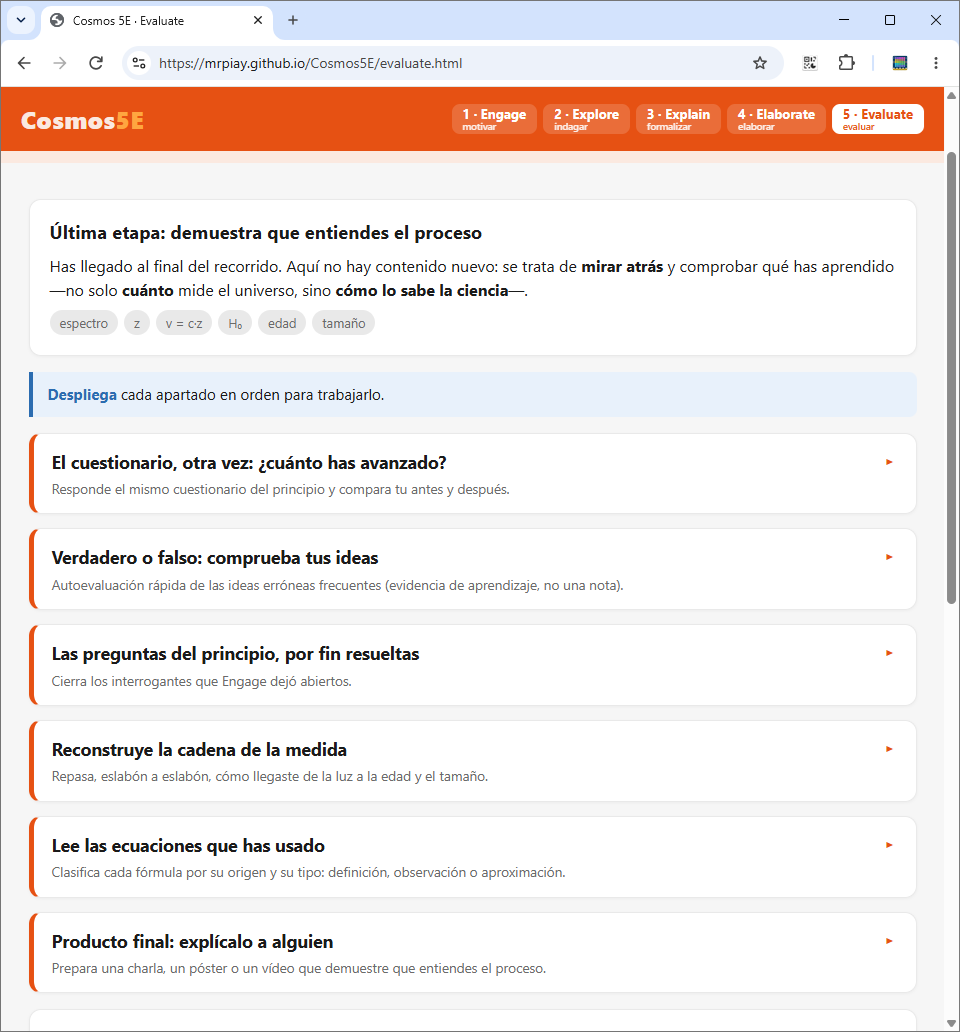
\includegraphics[width=0.82\textwidth]{./Images/web_v2_7_evaluate.png}
\caption{Captura de la sección \textbf{Evaluate} en la web interactiva.}\label{fig:web-evaluate}
\end{figure}

\section{Instrumentos y criterios de evaluación}\label{sec:instrumentos}

La evaluación combina un diseño \textbf{pre-post} de comprensión conceptual con \textbf{dos rúbricas} ---una del proceso de indagación y otra del producto final---, alineados con los objetivos OA1--OA7. El \textbf{cuestionario conceptual} consta de \textbf{15 ítems de opción múltiple} cuyos distractores recogen las seis ideas erróneas nucleares (§3.5) ---Big Bang como explosión puntual, universo con centro o borde, expansión de los sistemas ligados, corrimiento al rojo como Doppler ordinario, confusión entre materia y energía oscura, y energía oscura como «fuerza que empuja»---, junto con otras dificultades documentadas (interpretar $1/H_{0}$ como edad exacta, el radio observable como $c\times$edad, o la visión de la ciencia como conjunto de hechos cerrados). Se administra \textbf{sin cambios} antes (Engage) y después (Evaluate) para estimar la ganancia conceptual, con referente metodológico en \textcite{gasparini2025}. \textbf{Cada ítem se responde siempre} e incluye la opción \emph{«No lo sé / no lo tengo claro»} (para quien no lo tenga claro), de modo que el pre-test queda completo; es el mismo instrumento en ambos momentos. La medida comparable es el \textbf{número de aciertos}. Su versión completa y la clave de corrección se recogen en el anexo de instrumentos. Las \textbf{dos rúbricas} ---\textbf{A}, del trabajo de indagación de Explore, y \textbf{B}, del producto final--- fijan cuatro niveles de logro ---inicial\,(1), en proceso\,(2), adecuado\,(3) y avanzado\,(4)--- en cinco dimensiones cada una, con una \textbf{puntuación total} por suma de las cinco (de 5 a 20); ambas se detallan en el Anexo~\ref{cap:anexo-docente} (Tablas~\ref{tab:rubricaA} y~\ref{tab:rubricaB}).

Junto al cuestionario ---que \emph{mide} la ganancia conceptual pre-post--- y a las rúbricas, la fase Evaluate incorpora un \textbf{cuestionario de verdadero o falso} que confronta las ideas erróneas nucleares: es una \textbf{comprobación conceptual} que aporta \textbf{evidencia de aprendizaje} (autoevaluación con retroalimentación inmediata en la web), al margen del contraste pre-post.

Para facilitar la \textbf{recogida de datos} de la implementación prevista (curso 2026-2027), la web permite \textbf{exportar los resultados} de cada participante ---cuestionario pre y post, el $H_{0}$ medido, las conjeturas de Explore y la explicación de Explain--- en formato \textbf{CSV o JSON}, identificados únicamente con un \textbf{código anónimo} (sin nombres). Así, las respuestas que de otro modo quedarían solo en el almacenamiento local del navegador pueden recuperarse y analizarse con facilidad.

La web incorpora, además, un \textbf{modo de demostración}: rellena automáticamente todas las respuestas y reflexiones y desbloquea las cinco fases, de forma que el docente ---o cualquier persona que revise la herramienta--- puede \textbf{recorrer la secuencia completa sin tener que responder} y \textbf{exportar un conjunto de datos de ejemplo} (en CSV o JSON). Es una utilidad de \textbf{revisión y presentación}, ajena a la actividad del alumnado; su efecto se \textbf{revierte} al reiniciar la secuencia.

\section{Atención a la diversidad y adaptaciones}\label{sec:diversidad}

La secuencia contempla \textbf{andamiajes} y versiones de distinta demanda matemática, de modo que el objetivo central ---comprender el proceso de medida--- sea accesible a todo el alumnado con independencia de su soltura con el cálculo. Como garantía de equidad, cada actividad interactiva dispone de una \textbf{alternativa no digital} equivalente: el diagrama de Hubble puede construirse con datos en papel y una banda elástica que materialice el ajuste de la recta, y la calculadora puede seguirse paso a paso sobre una hoja de trabajo. Las adaptaciones concretas para necesidades específicas quedan \textit{[por concretar]} en función del grupo real.

\section{Plan de implementación (curso 2026-2027)}\label{sec:implementacion}

Se prevé implementar la secuencia en el curso 2026-2027, en un grupo de 2º de Bachillerato, a lo largo de siete sesiones. La recogida de datos pre-post permitirá analizar la ganancia conceptual y el tamaño del efecto, y valorar el cambio en las ideas erróneas. El plan atenderá a las consideraciones éticas oportunas ---información al alumnado, consentimiento y anonimato de los datos---. El grupo concreto, la temporalización definitiva y el detalle del análisis quedan \textit{[por concretar]}.

\subsection{Riesgos y amenazas a la validez}\label{sec:riesgos}

Aunque la validación empírica se difiere, conviene anticipar los principales \textbf{riesgos y amenazas a la validez} del futuro estudio pre-post, con sus mitigaciones:

\begin{itemize}
\item \textbf{Muestra pequeña y sin grupo de control} (un único grupo de aula): limita la validez externa y la inferencia causal. Se asume un carácter \textbf{exploratorio}; los resultados se interpretarán como indicios, no como evidencia concluyente.
\item \textbf{Doble rol docente--investigador} (el autor diseña, imparte y evalúa): posible sesgo del experimentador. Mitigación: uso de \textbf{instrumentos validados} (CosmoCI, \textit{construct map}) y criterios de corrección explícitos.
\item \textbf{Efecto test--retest y deseabilidad social} (mismos ítems antes y después): posible mejora artificial de las puntuaciones. Mitigación: separación temporal suficiente, anonimato de las respuestas y foco en el cambio conceptual, no en la calificación.
\item \textbf{Amenazas internas} (maduración, historia, instrumentación): otros contenidos o eventos del curso podrían influir. Mitigación: acotar la ventana temporal de la secuencia y registrar el contexto de implementación.
\item \textbf{Fidelidad de implementación}: que la secuencia se imparta tal como se diseñó. Mitigación: las fichas de fase y la web interactiva actúan como guion común.
\item \textbf{Dependencia tecnológica}: fallos de equipos o de conectividad. Mitigación: la web es \textbf{offline} (sin conexión) y cada actividad dispone de \textbf{alternativa en papel}.
\end{itemize}

Estas amenazas no invalidan la propuesta ---propia de un trabajo de \textbf{diseño}---, pero orientarán el diseño metodológico de la implementación del curso 2026-2027.

\section{Materiales de la secuencia (anexos)}\label{sec:materiales}

Los materiales de cada fase se han desarrollado como recursos de trabajo que, conforme a la propuesta de §4.1, integran la web interactiva; se incorporan como anexos, con sus enlaces y su atribución o licencia. La Tabla~\ref{tab:materiales} resume los materiales principales por fase.

\begin{table}[ht]
\centering
\caption{Materiales principales por fase.}\label{tab:materiales}
\begin{tabularx}{\textwidth}{|>{\raggedright\arraybackslash}p{2.4cm}|>{\raggedright\arraybackslash}X|}
\hline
\rowcolor{naranja}
{\color{white}\textbf{Fase}} & {\color{white}\textbf{Materiales principales}} \\ \hline
Engage & Reto y pregunta motriz; hitos de la línea de tiempo de la cosmología; simulación interactiva de la paradoja de Olbers; \textbf{cuestionario conceptual} de 15 ítems (con la opción «No lo sé / no lo tengo claro»), pre-test $=$ post-test. \\ \hline
Explore & Espectro(s) de trabajo para medir $z$; conjunto de datos del diagrama de Hubble (galaxias reales con distancia independiente del corrimiento al rojo y velocidad); herramienta de ajuste de recta (y su alternativa con banda elástica); formulario de \textbf{registro de la conjetura}. \\ \hline
Explain & Recogida de la \textbf{explicación del alumnado} (previa a la formalización); calculadora didáctica (cadena $z \rightarrow v \rightarrow H_{0} \rightarrow$ edad, con la conversión de unidades desplegada); gráfico «rebobinar la expansión»; recurso «el corrimiento al rojo de la luz»; calendario cósmico. \\ \hline
Elaborate & \textit{Parte 1 (tamaño):} calculadora (radio de Hubble), simulador del universo observable ($\sim$46\,000 millones de al) y actividad de \textbf{transferencia} a otros valores de $H_{0}$. \textit{Parte 2 (límites):} deslizador de la tensión de Hubble, ficha del modelo $\Lambda$CDM y sección sobre los horizontes. \\ \hline
Evaluate & Cuestionario \textbf{post} (mismos ítems que el pre, con corrección y contraste); \textbf{verdadero/falso} (evidencia de aprendizaje); actividad de lectura de las ecuaciones (apartado~\ref{sec:ecuaciones}); guion del producto final; \textbf{Rúbrica A} (Explore) y \textbf{Rúbrica B} (producto). \\ \hline
\end{tabularx}
\end{table}

\section{El modelo 5E como marco para discusiones abiertas}\label{sec:extension}

La secuencia principal culmina con la edad y el tamaño del universo, pero al determinar el tamaño aflora una pregunta más honda que ninguna fórmula cierra: ¿qué \textbf{forma} tiene el espacio? ¿Es finito o infinito, plano o curvo, y cómo podría saberse estando \textbf{dentro} de él? Esa pregunta ---abierta y sin respuesta de manual--- es el terreno idóneo para un uso distinto del modelo 5E: no como molde de una secuencia completa dirigida a una medida, sino como marco \textbf{breve y provocador} para una \textbf{discusión abierta}, cuyo objetivo no es dominar un contenido, sino despertar la curiosidad y hacer visibles las fronteras del conocimiento.

La lógica del 5E ---implicar, explorar, explicar, elaborar y evaluar--- funciona también \textbf{a menor escala}, en un ciclo corto de una o dos sesiones: se conserva el \textbf{motor} (partir de una provocación, indagar antes de formalizar y cerrar con una síntesis) y se relaja el \textbf{alcance} y, sobre todo, la \textbf{evaluación}, que se vuelve \textbf{formativa y reflexiva} ---el logro no es «acertar», sino formular buenas preguntas y reconocer los límites de lo que se sabe---. Un ejemplo natural de este uso, \textbf{opcional} y a modo de enriquecimiento ---fuera de la secuencia principal, por lo que no se incorpora a la web para no sobrecargarla---, sería un ciclo breve sobre la \textbf{geometría del universo}: partiendo del tamaño ya calculado, preguntar si el espacio es finito o infinito, plano o curvo; introducir la \textbf{densidad crítica} (con la lógica de la velocidad de escape) y distinguir el \textbf{destino} del universo (expansión eterna, límite o recolapso) de su \textbf{geometría} ---un resultado de la Relatividad General que se \emph{enuncia}, no se deduce, y cuyas ecuaciones pueden \emph{leerse} con la metodología del §\ref{sec:ecuaciones} y el Anexo~\ref{cap:anexo-ecuaciones}---. Aunque las medidas indican una curvatura \textbf{plana}, la discusión deja abiertas las grandes preguntas de fondo ---el tamaño total (¿finito o infinito?) y los modelos de expansión y destino---. Este formato resulta especialmente útil como \textbf{cierre} de la unidad o como estímulo de \textbf{vocaciones científicas} (OA7): la ciencia no termina en el resultado, sino que se abre en él, y el final de la secuencia principal se convierte en un principio.

\section{Las ecuaciones de la cosmología: metodología didáctica}\label{sec:ecuaciones}

Este apartado presenta una metodología didáctica para leer e interpretar ecuaciones y la aplica a las principales expresiones matemáticas utilizadas para estimar la edad y el tamaño del universo. Su objeto no es que el alumnado \emph{derive} dichas ecuaciones ---una tarea que excede el nivel de Bachillerato---, sino que aprenda a \emph{interpretarlas}: a comprender qué afirman, de qué dependen y qué tipo de conocimiento expresan.

Comprender la cosmología exige interpretar sus ecuaciones, que son el lenguaje en el que se expresa con exactitud el conocimiento científico: una relación como $v = H_{0}\,d$ es lo que convierte una observación ---el alejamiento de las galaxias--- en una estimación de la edad del universo. Sin embargo, para gran parte del alumnado de 2º de Bachillerato la ecuación constituye un obstáculo: los símbolos se manipulan mecánicamente ---se despejan, se sustituyen, se calculan--- sin llegar a interpretarse, y la fórmula acaba funcionando como una caja negra que produce resultados sin comprensión.

Esa dificultad suele afrontarse derivando las ecuaciones, es decir, reconstruyendo el razonamiento que conduce hasta ellas; pero en cosmología esa vía es inviable. Las expresiones fundamentales ---como las ecuaciones de Friedmann, la densidad crítica o la aceleración de la expansión--- proceden de la relatividad general. Sin embargo, no pueden omitirse, porque sostienen las magnitudes que la secuencia pretende estimar. Ante ecuaciones imprescindibles cuya derivación queda fuera del alcance del alumnado ---una circunstancia que hace de la cosmología un terreno idóneo para este enfoque---, el objetivo de aprendizaje se replantea: no derivarlas, sino aprender a leerlas e interpretarlas.

Con este fin se propone un \textbf{proceso de lectura} de seis etapas ---detallado más adelante--- que convierte el lenguaje simbólico en significado conceptual y culmina en la pregunta por el \emph{tipo} de conocimiento que la ecuación representa. El enfoque se apoya en la conversión entre registros semióticos \parencite{duval2006}, en la alfabetización matemática de PISA \parencite{oecd2019} y en la naturaleza de la ciencia \parencite{lederman1992}, y se integra en la secuencia 5E: cada ecuación que el alumnado emplea en las fases \emph{Explore}, \emph{Explain} y \emph{Elaborate} se analiza con el mismo procedimiento, fijo y repetible. El método se aplica, además, a las ecuaciones de fondo procedentes de la relatividad general ---las de Friedmann--- que sostienen el modelo pero que \textbf{no se calculan ni se derivan en el aula}: se \emph{leen} como ejemplo culminante del enfoque ---son, de hecho, sus únicos casos de tipo \emph{Derivación}---, no como contenido nuevo que el alumnado deba dominar. Así, comprender las fórmulas deja de ser un requisito implícito y se convierte en una tarea observable ---que puede plantearse, guiarse y calificarse---: un objetivo de aprendizaje explícito y evaluable, en el que las seis etapas funcionan como una rúbrica de comprensión.

\subsection{Las etapas del proceso de lectura}

El proceso de lectura se recorre en seis etapas, planteadas como preguntas que se formulan siempre en el mismo orden ante cualquier ecuación. Ese orden no es casual: conduce progresivamente desde la interpretación del lenguaje matemático hasta la valoración del tipo de conocimiento que expresa:

\begin{enumerate}
  \item \textbf{Símbolos.} ¿Qué representa cada símbolo y en qué unidades se expresa?
  \item \textbf{Relación.} ¿Cómo se vinculan las magnitudes entre sí? ¿La dependencia es directa, inversa\ldots?
  \item \textbf{Sentido.} ¿Qué indican los signos ---crecimiento, atracción, cancelación--- y qué significan? En las ecuaciones con varios términos, ¿cómo se leen en conjunto?
  \item \textbf{Propósito.} ¿Qué mide o predice la ecuación? ¿Para qué sirve?
  \item \textbf{Origen.} ¿De qué teoría o de qué observación procede? Se identifica su procedencia, sin reconstruir su derivación.
  \item \textbf{Tipo.} ¿Qué clase de afirmación es la ecuación?
\end{enumerate}

La sexta pregunta se responde clasificando la ecuación en una de cuatro categorías, que precisan la naturaleza del conocimiento que expresa y el grado de confianza que puede atribuírsele:

\begin{itemize}
  \item \textbf{Definición.} La ecuación se limita a nombrar o convenir una magnitud; no se demuestra, se establece.
  \item \textbf{Observación.} Expresa un patrón medido en la naturaleza, no deducido de una teoría; su validez descansa en los datos.
  \item \textbf{Aproximación.} Es válida únicamente bajo ciertas condiciones, que deben explicitarse; fuera de ellas deja de aplicarse.
  \item \textbf{Derivación.} Se obtiene de una teoría más general; no se reconstruye aquí su derivación, pero se identifica su origen.
\end{itemize}

Las cinco primeras preguntas permiten interpretar el contenido matemático de la ecuación; la sexta desplaza la atención desde lo que la ecuación dice hacia la razón por la que puede aceptarse como conocimiento científico.

\subsection{Un ejemplo: la ley de Hubble}

A modo de ilustración, el proceso se aplica a la ley de Hubble-Lemaître, $v = H_{0}\,d$, ecuación central de la secuencia:

\begin{itemize}
  \item \textbf{Símbolos.} $v$ es la velocidad de recesión de una galaxia (km/s); $d$, su distancia (Mpc); $H_{0}$, la constante de Hubble (km/s por Mpc).
  \item \textbf{Relación.} Directa: cuanto mayor es la distancia, mayor es la velocidad de alejamiento.
  \item \textbf{Sentido.} La velocidad de recesión es positiva y crece con la distancia para las galaxias suficientemente lejanas; en $d = 0$ resulta $v = 0$: no hay recesión respecto del propio observador.
  \item \textbf{Propósito.} Representada gráficamente para muchas galaxias, la pendiente de la recta proporciona el valor de $H_{0}$, a partir del cual se estima después la edad del universo.
  \item \textbf{Origen.} Es una \textbf{relación empírica}: el patrón que Hubble observó en 1929 al relacionar la velocidad y la distancia de las galaxias; es, además, consistente con los modelos cosmológicos homogéneos de expansión.
  \item \textbf{Tipo.} \emph{Observación.} Es un hecho empírico; interpretar que implica la expansión del universo constituye una lectura del modelo cosmológico, no una consecuencia lógica de la fórmula.
\end{itemize}

Esta lectura transforma una ecuación que el alumnado tendería simplemente a «usar» ---despejar $H_{0}$, sustituir valores--- en una afirmación que comprende: sabe qué relaciona, para qué sirve, de dónde procede y qué alcance tiene. El anexo~\ref{cap:anexo-ecuaciones} recoge esta lectura para las nueve ecuaciones de la cosmología: las cinco que vertebran la medida en la secuencia y las cuatro de fondo ---las de Friedmann--- que allí solo se leen, sin derivarlas.
